\message{ !name(paper.tex)}%  article.tex (Version 3.3, released 19 January 2008)
%  Article to demonstrate format for SPIE Proceedings
%  Special instructions are included in this file after the
%  symbol %>>>>
%  Numerous commands are commented out, but included to show how
%  to effect various options, e.g., to print page numbers, etc.
%  This LaTeX source file is composed for LaTeX2e.

%  The following commands have been added in the SPIE class 
%  file (spie.cls) and will not be understood in other classes:
%  \supit{}, \authorinfo{}, \skiplinehalf, \keywords{}
%  The bibliography style file is called spiebib.bst, 
%  which replaces the standard style unstr.bst.  

\documentclass[]{spie}  %>>> use for US letter paper
%%\documentclass[a4paper]{spie}  %>>> use this instead for A4 paper
%%\documentclass[nocompress]{spie}  %>>> to avoid compression of citations
%% \addtolength{\voffset}{9mm}   %>>> moves text field down
%% \renewcommand{\baselinestretch}{1.65}   %>>> 1.65 for double spacing, 1.25 for 1.5 spacing 
%  The following command loads a graphics package to include images 
%  in the document. It may be necessary to specify a DVI driver option,
%  e.g., [dvips], but that may be inappropriate for some LaTeX 
%  installations. 
\usepackage{graphicx}
\usepackage{subfig}
\usepackage{amsmath}
\usepackage{amssymb}
\usepackage{hyperref}
\usepackage{float}
\title{Texture mapping 3D planar models of indoor environments with noisy camera poses} 

%>>>> The author is responsible for formatting the 
%  author list and their institutions.  Use  \skiplinehalf 
%  to separate author list from addresses and between each address.
%  The correspondence between each author and his/her address
%  can be indicated with a superscript in italics, 
%  which is easily obtained with \supit{}.

\author{Peter Cheng, Michael Anderson, Stewart He, Avideh Zakhor
\skiplinehalf
University of California, Berkeley\\
}

 

%%%%%%%%%%%%%%%%%%%%%%%%%%%%%%%%%%%%%%%%%%%%%%%%%%%%%%%%%%%%% 
%>>>> uncomment following for page numbers
% \pagestyle{plain}    
%>>>> uncomment following to start page numbering at 301 
%\setcounter{page}{301} 
 
\begin{document}

\message{ !name(paper.tex) !offset(395) }
\subsection{Image Occlusion}
\label{sec:imageOcclusion}

\begin{figure}
  \centering
  \subfloat[][]{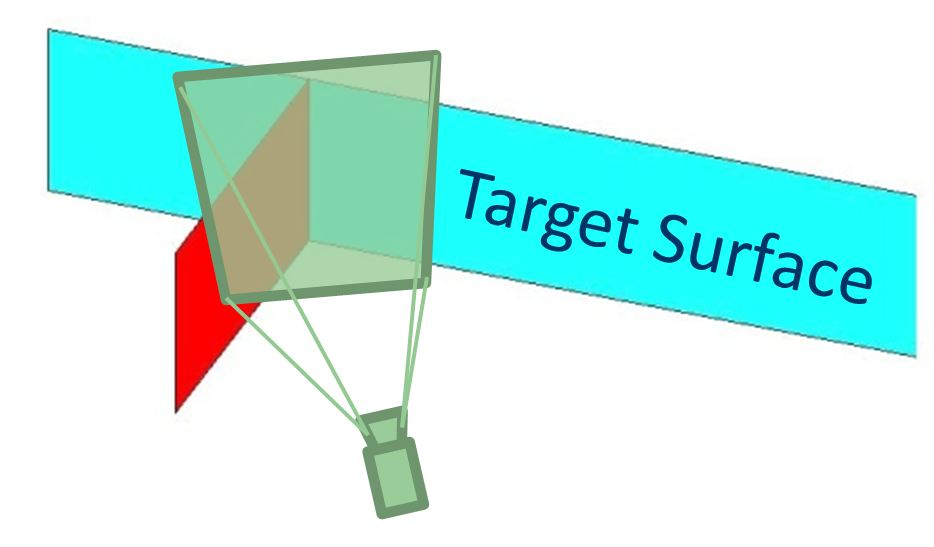
\includegraphics[width=3in]{occlusiondiagram.jpg}}
  \hspace{0.4cm} \subfloat[][]{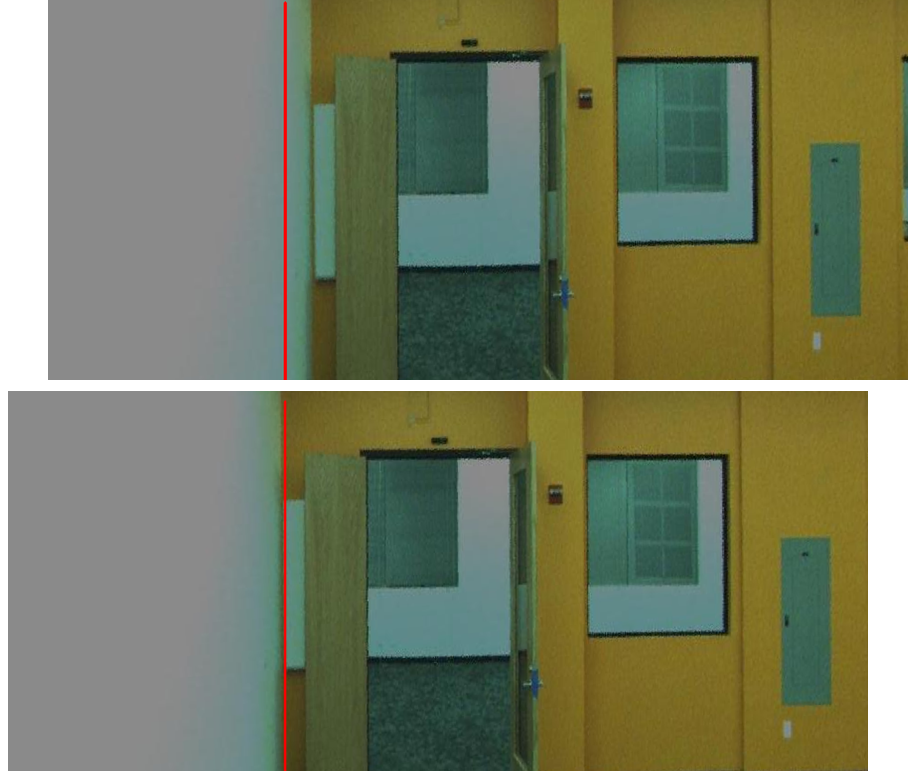
\includegraphics[width=3in, height=1.8in]{occlusionimages.png}}
  \caption{(a) The green image contains texture that belongs to the red surface, which should not be projected onto the blue target surface. (b) Above, without geometry alignment, texture to the left of the red line would be removed, which would leave some erroneous texture projected onto our target surface. Below, after geometry alignment, the correct amount of texture is removed.}
  \label{fig:occlusion}
\end{figure}

In order to properly texture surfaces such as the one shown in Figure
\ref{fig:occlusion}, it is important to detect when parts of image
projections contain texture belonging to other surfaces and should
therefore not be used. This can be tested by recursively performing
ray-polygon intersection tests between camera locations and other
surfaces in a regularly spaced grid \cite{rayintersection}. Where four
corners of a rectangular region are occluded, texture is
removed. Where no corners are occluded, the recursion stops. Where
there is a mixture of both, the rectangular region is subdivided into
four, and the same process is performed on each. By performing Section
\ref{sec:geometryAlignment}'s alignment procedure before occlusion,
texture belonging to other surfaces is accurately removed, which is
necessary for the next section.

\message{ !name(paper.tex) !offset(791) }

\end{document} 
